% ########################################################################################################################################
%
% This is the main latex file. Here we call for inputs from other files. We also define some of the main characteristics of the document.
%
% ########################################################################################################################################
%
% You likely only need to modify the "Main_Content__Write_your_essay_here.tex" file.
%
% ########################################################################################################################################

\documentclass[12pt,a4paper,oneside]{paper}
% Encoding and Language
\usepackage[utf8x]{inputenc}
\usepackage{csquotes}
\usepackage[main=english,portuguese]{babel}
\usepackage{iflang}
\usepackage{ragged2e}
\usepackage{makeidx}
\usepackage{multicol}
\usepackage[export]{adjustbox}
\usepackage{tikz-dependency}
\usepackage{fancyhdr}

% Font Configurations
\renewcommand{\rmdefault}{phv}
\renewcommand{\sfdefault}{phv}
\def\FontLn{% 16 pt normal
  \usefont{T1}{phv}{m}{n}\fontsize{16pt}{16pt}\selectfont}
\def\FontLb{% 16 pt bold
  \usefont{T1}{phv}{b}{n}\fontsize{16pt}{16pt}\selectfont}
\def\FontMn{% 14 pt normal
  \usefont{T1}{phv}{m}{n}\fontsize{14pt}{14pt}\selectfont}
\def\FontMb{% 14 pt bold
  \usefont{T1}{phv}{b}{n}\fontsize{14pt}{14pt}\selectfont}
\def\FontSn{% 12 pt normal
  \usefont{T1}{phv}{m}{n}\fontsize{12pt}{12pt}\selectfont}

% Font Encoding
\usepackage[T1]{fontenc}

% Page Geometry
\usepackage{geometry}	
\geometry{verbose,tmargin=2.cm,bmargin=2.cm,lmargin=2.cm,rmargin=2cm}

% Line Spacing
\usepackage{setspace}
\renewcommand{\baselinestretch}{1.25}

% Graphics and Figures
\usepackage{graphicx}
\usepackage{subfigure}
\usepackage{subfigmat}
\usepackage{float}

% Mathematics and Theorems
\usepackage{amsmath}
\usepackage{amsthm}
\usepackage{amsfonts}
\usepackage{dcolumn}
\usepackage{indentfirst}

% Comments and Verbatim
\usepackage{verbatim}

% Hyperlinks
\usepackage[pdftex]{hyperref}
\hypersetup{
    colorlinks,
    linkcolor=blue,
    anchorcolor=black,
    citecolor=cyan,
    filecolor=black,
    menucolor=black,
    urlcolor=teal,
    bookmarksopen=true,
    bookmarksnumbered=true
}

% Captions and References
\usepackage[figure,table]{hypcap}
\usepackage[format=plain]{caption}
\DeclareCaptionFont{georgia}{\small\fontseries{n}\fontfamily{georgia}\selectfont}
\captionsetup{labelfont=georgia,font=georgia}

% Bibliography
\usepackage[backend=biber,style=apa]{biblatex}

% Acronyms
\usepackage[printonlyused]{acronym}

% Lipsum (for placeholder text)
\usepackage{lipsum}

% Cleveref (for clever references)
\usepackage[\IfLanguageName{english}{english}{portuguese}]{cleveref}

% Colors
\usepackage{xcolor}
\usepackage{color}

% Custom Commands
\newcommand{\gray}[1]{\textcolor{gray}{#1}}

% Equation Numbering
\renewcommand{\theequation}{{\fontseries{n}\fontfamily{georgia}\selectfont\arabic{equation}}}

% Section and Subsection Fonts
\sectionfont{\Large\bfseries\fontfamily{lmss}\selectfont}
\subsectionfont{\large\bfseries\fontfamily{lmss}\selectfont}

\makeindex

\addbibresource{bibliography.bib}
\begin{document}
\pagestyle{plain}

%TC:ignore
% #############################################################################
%
%                           ENTER YOUR NAME, ISTid, AND TITLE
% 
% #############################################################################



\def\title {}


% #############################################################################
%
%               DO NOT MODIFY THE LINES FROM HERE TO THE MAIN DOCUMENT BODY
% 
% #############################################################################

\thispagestyle {empty}
\begin{center}
\begin{minipage}[c][5cm][t]{\textwidth}
\begin{center}
\includegraphics[width=5cm]{../IST_A_RGB_POS.png}
\end{center}

\end{minipage}
\begin{minipage}[t][10cm][c]{\textwidth}
\centering
{\FontMb Laboratório de Introdução à Física Experimental} \\
\paragraph{}
\centering
{\FontLb\Huge \title{Experiência de Milikan}}
\paragraph{}
{\FontMb Estimativa da carga elétrica de gotículas de óleo eletrizadas em suspensão num fluido} \\
\paragraph{}
{\FontMb 2023}
\end{minipage}

\begin{minipage}[c][1.5cm][c]{\textwidth}
\centering
{\FontLn }
\end{minipage}

\begin{minipage}[c][1.5cm][c]{\textwidth}
\centering



\end{minipage}
\begin{minipage}[c][3cm][c]{\textwidth}
\centering
\renewcommand{\arraystretch}{1.4}

\maketitle

\vspace{-5mm}
\hline
\vspace{-3mm}
\begin{center}
\centering
\section*{\centering Objetivos}
    \vspace{-3mm}
\small
\justify
Pretende-se com este trabalho determinar a carga eléctrica de pequenas gotas de óleo, tendo como objetivo final mostrar que a carga eléctrica não aparece com uma quantidade qualquer mas sempre como um múltiplo de uma unidade fundamental: a carga do electrão. Deste modo, um corpo electrizado apresenta um excesso de carga de sinal positivo ou negativo, mas cuja valor é sempre um múltiplo do valor da carga elementar $q_{ele}= 1,602176634\cdot 10^{-19}\,$ C.
Traduz-se este facto dizendo-se que a carga eléctrica é \emph{quantizada}.

Dentro das várias experiências elaboradas para mostrar este facto, uma montagem clássica é a do físico americano Robert A. Millikan\footnote{Millikan recebeu o prémio Nobel da Física em 1923 pelos seus trabalhos sobre a determinação da carga do electrão e efeito fotoeléctrico.} (1869-1953), também chamada experiência da gota de óleo.
    
\end{center}
\hline


\end{minipage}
\begin{minipage}[c][2cm][c]{\textwidth}
\centering

\end{minipage}

\end{center} 
\normalsize
\cleardoublepage
\setcounter{page}{1}
\fontfamily{cmr}\selectfont
%TC:endignore
% #############################################################################
%
%                           BEGIN MAIN DOCUMENT BODY
%
% #############################################################################

\printindex


\section{\sf Conceitos fundamentais}
\subsection{\sf Traçado de raios}
A ótica geométrica, ou ótica de raios, é uma abordagem que consiste em descrever a propagação da luz através de raios.
Um raio é um modelo simplificado, na forma de uma linha, que descreve o caminho percorrido pela luz entre duas superfícies.
Para descrever a propagação de um feixe de luz através de um sistema, utilizamos um conjunto de raios, que se propagam utilizando
o método do \emph{traçado de raios}.
Este método é suficiente para explicar fenómenos como a reflexão e a refracção da luz e é particularmente útil na descrição
de sistemas e instrumentos óticos, sendo válida desde que as dimensões dos objetos envolvidos sejam muito maiores que o c.d.o.
da luz visível ($\sim$ 0,4 a 0,7 $\mu$m).

O comportamento dos raios obedece a algumas regras simples:

\begin{enumerate}
\item Num meio uniforme, como o ar ou um vidro, um raio é uma linha recta;
\item Um meio ótico é definido por uma grandeza $n\geq1$, chamada índice de refracção;
\item Na fronteira entre dois meios, um raio é reflectido e/ou refractado, verificando-se:
\begin{itemize}
\item o ângulo de reflexão é igual ao ângulo de incidência
\item o ângulo de refracção $\theta_r$ e o ângulo de incidência $\theta_i$ (medidos relativamente à normal à superfície)
obedecem à \emph{Lei de Snell-Descartes},

\begin{equation}
n_i\sin{\theta_i}=n_r\sin{\theta_r}
\end{equation}
em que $n_i$ e $n_r$ são respectivamente os índices de refracção do meio de incidência e do meio de refracção.
\end{itemize}
\end{enumerate}
%%%%%%%%%%%%
\begin{figure}
\begin{center}
	\includegraphics[width=0.4\textwidth]{./otica_images/1-snell}
	\caption{Raio reflectido e refractado na fronteira entre dois meios.}
	 \label{fig:snell}
\end{center}
\end{figure}
%%%%%%%%%%%%

\subsection{\sf Reflexão, refracção e polarização}

A eficiência com que um feixe luminoso é reflectido ou refractado numa fronteira entre dois meios de índices de refracção
$n_1$ e $n_2$ depende, entre outros, do ângulo de incidência e da polarização da luz. A Fig. \ref{fig:brewster} mostra como
varia a reflectividade de uma superfície de vidro em função do ângulo de incidência, para polarizações horizontal e vertical
(admitindo que o plano de incidência e reflexão é horizontal). Para um ângulo específico, designado \emph{ângulo de Brewster}
e dado por $\theta_B=\arctan(n_2/n_1)$, a componente horizontal da polarização não é reflectida, pelo que a luz reflectida fica
com polarização vertical. Esta é uma forma de criar luz polarizada a partir de uma fonte não-polarizada. A figura ilustra também
a geometria dos raios luminosos numa separação entre dois meios, no caso de incidência em ângulo de Brewster. Como se pode apreciar,
nessa configuração o raio reflectido e o raio refractado fazem entre si um ângulo de 90$^\circ$.

Pode-se polarizar a luz emitida por uma fonte não-polarizada através de um simples filtro polarizador (ou \textit{polaroide}).
Orientando o ângulo do filtro relativamente à direcção dos raios luminosos, é possível definir a direcção de polarização
(Fig. \ref{fig:pol-luz}).

%%%%%%%%%%%%
\begin{figure}[H]
\begin{center}
	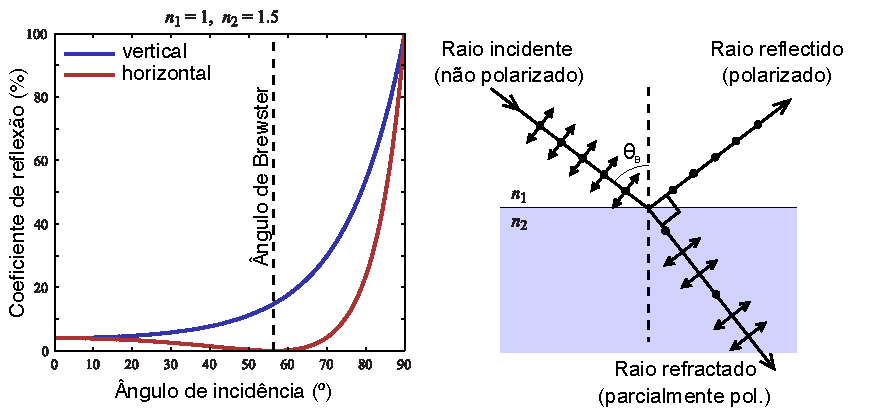
\includegraphics[width=0.85\textwidth]{./otica_images/2-brewster}
	\caption{Reflectividade vs. ângulo de incidência e direcção de polarização (esq.) e geometria para ângulo de Brewster
    (dir.). \label{fig:brewster}} 
\end{center}
\end{figure}
%%%%%%%%%%%%

\begin{figure}[H]
\centering 
	\includegraphics[width=0.8\textwidth]{./otica_images/2-pol-luz}
	\caption{Obtenção de luz polarizada (verticalmente, no caso da figura) através de um filtro polarizador. \label{fig:pol-luz}} 
\end{figure}






%%%%%%%%%%%%%%%%%%%%%%%%%%%%%%%%%%%%%%%%%%%%%%%%%%
%%%%%%%%%%%%%%%%%%%%%%%%%%%%%%%%%%%%%%%%%%%%%%%%%%
\section{\sf Construções geométricas em lentes delgadas}

Uma das principais aplicações da ótica geométrica consiste no estudo da formação de imagens: dado um \emph{objeto} numa
dada posição, como desenhar um sistema ótico que permita transferir uma \emph{imagem} desse objeto para uma posição diferente?
É um problema que tem aplicações desde o olho humano até ao desenho de lentes e fibras óticas.

 Um \emph{objeto} iluminado uniformemente é considerado como uma fonte de raios, emitidos em todas as direcções. Podemos
 escolher um ponto no objeto e um conjunto adequado de raios, e traçar o seu percurso através do sistema até encontrar o
 correspondente ponto na \emph{imagem}. Por convenção, desenha-se o sistema ótico em torno de um eixo, que coincide com
 o seu eixo geométrico, e os raios propagam-se da esquerda para a direita. 



\subsection{\sf Aproximações}
Utilizaremos as duas seguintes aproximações comuns, que facilitam grandemente os cálculos a efectuar (Fig. \ref{fig:fig2}):

\emph{Lentes delgadas} -- uma lente é considerada \emph{delgada} quando a sua espessura $d$ é desprezável face à sua distância
focal $f$.

\emph{Aproximação paraxial} -- admitimos que todos os raios envolvidos são \emph{paraxiais}, isto é, (\emph{i}) situam-se
próximo do eixo ótico e (\emph{ii}) o ângulo $\alpha$ que fazem com esse eixo permite utilizar as aproximações
$\sin \alpha \approx \alpha$ e  $\tan \alpha \approx \alpha\,$, tipicamente válidas para $\alpha \leq  5^{\circ}$.

\begin{figure}[H]
	\centering 
	\includegraphics[width=0.4\textwidth]{./otica_images/2-definicoes}
 	\caption{\label{fig:fig2} Definições utilizadas: $f$ -- distância focal, $d\ll f$ -- espessura da lente delgada, $\alpha$ --
    ângulo entre o raio e o eixo ótico.} 
\end{figure}



%%%%%%%%%%%%%%%%%%%%%%%%%%%%%%%%%%%%%%%%%%%%%%%%%%
\subsection{\sf Convenções}
A Fig. \ref{fig:convencoes} ilustra os principais parâmetros do traçado de raios através de uma lente simples.

\begin{itemize}
\item O objeto $AB$ fica (por definição) do lado esquerdo da lente, a uma distância $d_O>0$ desta; caso o objeto esteja
do lado direito, temos $d_O<0$ (que é o caso do "objeto virtual" abordado mais à frente)
\item A imagem $A'B'$ está do lado direito da lente, a uma distância $d_I>0$ desta; caso a imagem esteja do lado esquerdo,
temos $d_I<0$
\item $F_0$ é a distância focal do lado do objeto, $F_I$ é a distância focal do lado da imagem. No caso de uma lente fina,
ambas são iguais a $f$, e marcam-se para auxiliar no traçado.
\end{itemize}

\begin{figure}[H]
	\centering 
	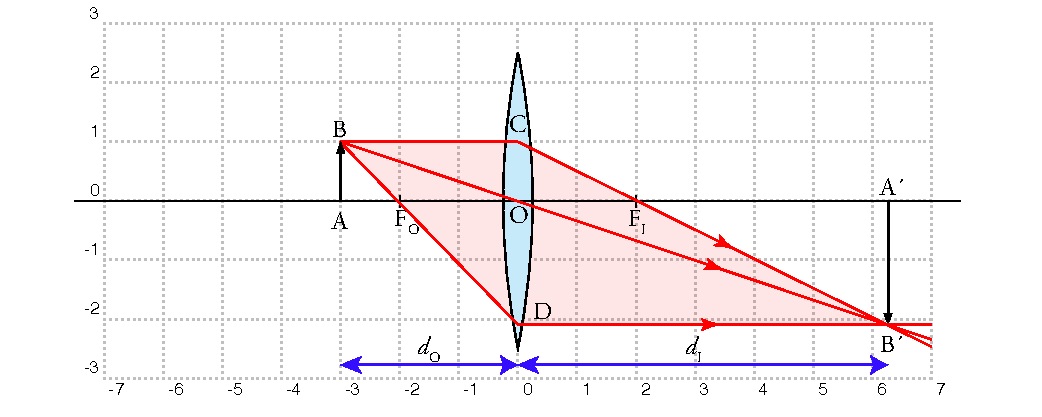
\includegraphics[width=0.9\textwidth]{./otica_images/3-convencoes}
	\caption{Convenções utilizadas para formação de imagens por lentes. \label{fig:convencoes}} 
\end{figure}

O raios óticos que emergem de um dado objeto atravessam a lente e dão origem a uma imagem. As imagens dizem-se \emph{reais}
quando os raios de luz passam de facto na posição da imagem, isto é, raios que saem do plano do objeto convergem no plano da
imagem; e dizem-se \emph{virtuais} quando os raios não passam na imagem, mas esta é visível através da lente. As imagens reais
podem ser projectadas num alvo, as virtuais não. Um bom exemplo é considerar a imagem de uma lâmpada brilhante: ao passar a mão
pelo plano da imagem, se estar for real sente-se o calor, mas se for virtual parecerá apenas "flutuar" no espaço.

De seguida, vamos analisar a formação de imagens para lentes convergentes ($f>0$) e divergentes ($f<0$) em função da posição
relativa do objeto e do foco da lente, e derivar relações úteis para lentes delgadas.



%%%%%%%%%%%%%%%%%%%%%%%%%%%%%%%%%%%%%%%%%%%%%%%%%%
\subsection{\sf objeto e imagem - focos conjugados e ampliação transversal}
Considere de novo a Fig. \ref{fig:convencoes}. Cada ponto do objeto em $d_O$ tem um único ponto correspondente na imagem
em $d_I$. Isto implica que, caso colocássemos o objeto em $d_I$, a imagem seria formada em $d_O$. Chama-se a estas posições
\emph{focos conjugados}.
Pela semelhança de triângulos temos as seguintes relações entre as dimensões do objeto e da imagem:

\begin{IEEEeqnarray}{rClrCl}
%\begin{array}{ccccc}
\Delta ABF_O \sim \Delta ODF_O  &\to & AB/A'B' = AF_O / F_O 0 &\to & AB/A'B' =  \frac{d_O-f}{ f} \label{eq:1} \\
\Delta ABO\sim \Delta A'B'O    &\to & AB/A'B' = AO / O A' &\to & AB/A'B' = d_O / d_I \label{eq:2} \\
\Delta COF_I \sim \Delta A'B'F_I  &\to & AB/A'B' = OF_I / F_I A' &\to & AB/A'B' =  \frac{f}{ d_I-f} \label{eq:3} 
\end{IEEEeqnarray}

Das expressões (\ref{eq:1}) e (\ref{eq:3}) obtemos a equação dos focos conjugados:
 
 \begin{equation}
	\label{eq:focosconjug}
    \fbox{
        $ \displaystyle
	\frac{1}{f} = \frac{1}{d_O} +\frac{1}{d_I} 
        $
    }
% \qquad \text{ equação dos focos conjugados}
\end{equation}

Uma forma alternativa e muitas vezes conveniente de exprimir esta relação consiste em utilizar as distâncias do objeto
e da imagem aos respectivos focos. Designando estas distâncias por $x_O=AF_O$ e $x_I=A'F_I$, tem-se $d_O=f+x_O$ e $d_I=f+x_I$.
Substituindo na expressão acima, obtém-se a chamada formulação de Newton para a equação dos focos conjugados:

 \begin{equation}
	\label{eq:focosconjugnewton}
    \fbox{
        $ \displaystyle
	x_Ox_I = f^2
        $
    }
% \qquad \text{ equação dos focos conjugados}
\end{equation}

Por outro lado, sendo $AB$ e $A'B'$ respectivamente as dimensões lineares transversais do objeto e da imagem, usamos a
igualdade (\ref{eq:2}) para definir a \emph{ampliação transversal} $A$ como:

 \begin{equation}
    \fbox{
        $ \displaystyle
A =  \frac{A'B'}{ AB} =\frac{d_I}{d_O}
$
}
\end{equation}
 
A imagem é \emph{direita} se $A<0$ e \emph{invertida} se $A>0$. Podemos usar estas duas equações para, dados $f$ e $d_O$,
determinar as seguintes expressões para a posição da imagem $d_I$ e a respectiva ampliação $A$:
 
\begin{eqnarray}
A&=&\frac{1}{\frac{d_O}{f}-1}\\
d_I&=&d_OA
\end{eqnarray}

 
Como exemplo, temos no caso da Fig. \ref{fig:convencoes}: $d_O>f \to A> 0\,; d_I > 0$. A imagem resultante é \emph{real}
e \emph{invertida}.

%%%%%%%%%%%%%%%%%%%%%%%%%%%%%%%%%%%%%%%%%%%%%%%%%%
\subsubsection{\sf Lente convergente ($f>0$) -- Imagem real}
Este caso verifica-se para $d_O>f$, a imagem é real é pode ser projectada. A imagem é menor ($A<1$) que o objeto se $d_O>2f$
ou maior ($A>1$) se $2f>d_O>0$. Um exemplo do primeiro caso é uma máquina fotográfica: a imagem é posicionada no sensor da câmara,
e é (tipicamente) menor que o objeto fotografado. Verifica-se  \fbox{$0 < A \le 1$ } pois

\begin{equation}
\infty > d_O \ge 2 f \quad \to \quad f < d_I \le 2 f  \quad \to \quad 0<A\le 1
\end{equation}

Um exemplo do segundo caso é um projetor de cinema ou de imagem de computador: a imagem é posicionada num écran, e é maior
que o objeto (película ou chip). Verifica-se  \fbox{$1 \le A < \infty$} pois

\begin{equation}
f < d_O \le 2 f  \quad \to  \quad  \infty > d_I \ge 2f \quad \to \quad \infty>A\ge 1
\end{equation}

%%%%%%%%%%%%%%%%%%%%%%%%%%%%%%%%%%%%%%%%%%%%%%%%%%
\subsubsection{\sf Lente convergente ($f>0$) -- Imagem virtual}

Este caso verifica-se quando $d_O<f$, por exemplo quando utilizamos uma lupa para ver objetos com um tamanho aumentado,
e está esquematizada na Fig. \ref{fig:fig4}. Dependendo da posição $d_O$, verificam-se as seguintes relações

%\begin{figure}
%	[!htb]  \centering 
%	\includegraphics[width=0.8 \textwidth]{lupa}
%	\caption{. \label{fig:lupa}} 
%\end{figure}

\begin{IEEEeqnarray}{rCl}
0 < d_O \le \frac{f}{2} \qquad & 0 > d_I \ge -f \quad& -1 >A \ge -2\\
\frac{f}{2} \le d_O < f \qquad& -f\ge d_I >-\infty \quad& -2 > A > -\infty
\end{IEEEeqnarray}

Repare-se que resulta $d_I<0$ (a imagem está do mesmo lado que o objeto) e $A<0$ pelo que a imagem é (\emph{i}) virtual
e (\emph{ii}) direita, para um observador colocado à direita da lente.

% \begin{figure}
%     \begin{center}
%     \psscalebox{0.75}{
%     \begin{pspicture}[showgrid=true](-7,-3)(7,3)
%     \rput(0,0){\lens[lensType=CVG,focus=4.5,OA=-2.7,AB=1,XO=0,YO=0,nameF=F_O,nameFi=F_I,spotAi=0,drawing=true,rayColor=white]}
%     \psline[linecolor=red,linestyle=dashed](B')(F')
%     \psline[linecolor=red,linestyle=dashed](B')(B)
%     \psline[linecolor=red](B)(0,1)
%     \psline[linecolor=red](B)(2.7,-1)
%     \psline[linecolor=red](0,1)(F')
%     \psset{linecolor=red}
%     \Arrows[posStart=0,length=1](B)(0,1)
%     \Arrows[posStart=2,length=3](B)(0,0)
%     \Arrows[posStart=0,length=3](0,1)(F')
%     \rput(8,0){\psset{linecolor=black}\eye}
%     \end{pspicture}
%     }
%     \caption{Formação de imagem virtual com uma lente convergente. \label{fig:fig4}} 
%     \end{center}
% \end{figure}

%%%%%%%%%%%%%%%%%%%%%%%%%%%%%%%%%%%%%%%%%%%%%%%%%%



\begin{figure}[H]
 \centering 
	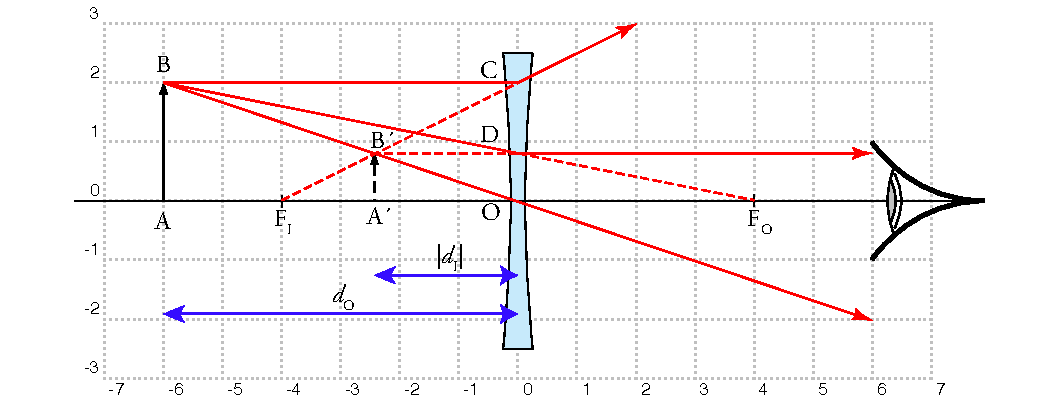
\includegraphics[width=0.7\textwidth]{./otica_images/5-DivVirt}
	\caption{Formação de imagem virtual com uma lente divergente. \label{fig:DivVirt}} 
\end{figure}

\subsubsection{\sf Lente divergente ($f<0$)}
Considere-se a situação representada na Fig. \ref{fig:DivVirt}, que mostra uma lente divergente ($f<0$) e um objeto 
$AB$ ($d_O>0$). Note-se que, no caso da lente divergente, os pontos $F_O$ e $F_I$ trocam de posição. Nesta configuração a
imagem resultante $A'B'$ é sempre \emph{virtual}  e \emph{direita} com $d_I <0$ (imagem do mesmo lado do objeto), pois

\begin{equation*}
f<0; \quad d_O> 0 \quad \to  \quad A<0;  \quad  d_I <0  
\end{equation*}

Podemos verificar que a equação (\ref{eq:focosconjug}) se mantém válida neste caso, recorrendo à semelhança de triângulos:
\begin{IEEEeqnarray}{rClrCl}
%\begin{array}{ccccc}
\Delta ABO \sim  \Delta A'B'O  & \to & AB/A'B' = \frac{d_0}{d_I} & \to & -\infty < A < 0 \label{eq:diver1} \\
\Delta ABF_0\sim \Delta ODF_O   &\to & \frac{d_0 + |f|}{|f|} = AB/A'B' & \to & \frac{d_0 + |f|}{|f|} = \frac{d_0 }{d_I}  \label{eq:diver2} \\
\Delta F_I OC \sim \Delta F_I A'B'  &\to & \frac{|f|}{|f| - |d_I|} =AB/A'B'  &  \to &  \frac{|f|}{|f| - |d_I|} = \frac{d_0 }{|d_I|} 
\end{IEEEeqnarray}

Nestas expressões, que descrevem distâncias, foi necessário  utilizar os valores em módulo de $f$ e de $d_I$, que são ambos
negativos. Fazendo agora as substituições $|f|\to -f$ e $|d_I|\to -d_I$ recupera-se a equação dos focos conjugados.


%%%%%%%%%%%%%%%%%%%%%%%%%%%%%%%%%%%%%%%%%%%%%%%%%%
\subsection{\sf objetos virtuais}

Em determinadas situações, podemos lidar com "objetos virtuais"  ($d_O<0$), isto é, os raios óticos têm origem não num
objeto sólido, mas num plano do espaço, e estamos interessados em estudar a sua propagação a partir desse plano e a formação
da imagem correspondente. Um exemplo típico consiste em estudar a formação da imagem de uma imagem primária. Nestes casos, o
objeto virtual é identificado a tracejado no diagrama de raios, como ilustrado nos exemplos em baixo.

%%%%%%%%%%%%%%%%%%%%%%%%%%%%%%%%%%%%%%%%%%%%%%%%%%
\subsubsection{\sf Lente convergente $f>0$}
A Fig. \ref{fig:ConvVirt} representa um objeto virtual ($d_O<0$, à direita da lente) e a correspondente imagem. A imagem
resultante é real ($d_I>0$, também à direita) e direita ($A<0$), verificando-se

\begin{IEEEeqnarray}{rCl}
 d_O < 0 ; \quad &&  f > 0 \quad \to \quad A<0  \nonumber\\
\frac{d_I}{-|d_O|}  & =&  \frac{f}{-|d_O| -f}     \nonumber
\end{IEEEeqnarray}



\begin{figure}[H]
 \centering 
	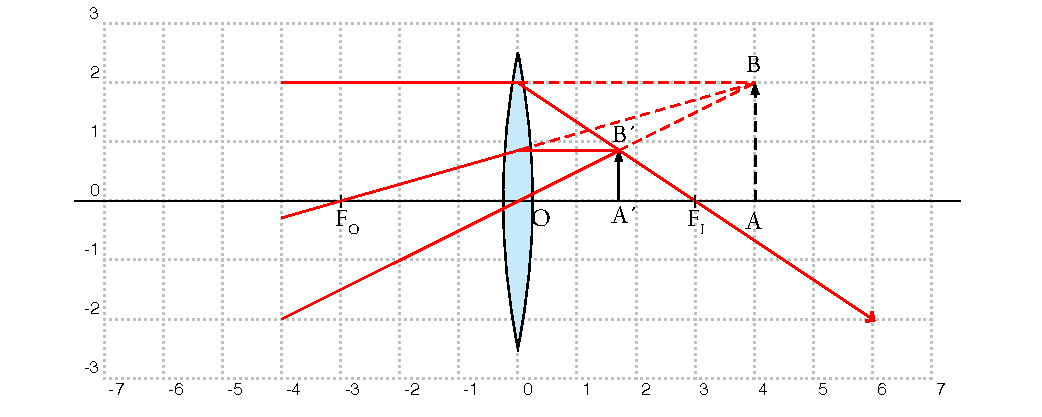
\includegraphics[width=0.7\textwidth]{./otica_images/6-ConvVirt}
	\caption{Lente convergente com objeto virtual e imagem real. \label{fig:ConvVirt}} 
\end{figure}

%%%%%%%%%%%%%%%%%%%%%%%%%%%%%%%%%%%%%%%%%%%%%%%%%%



\begin{figure}[H]
	\centering 
	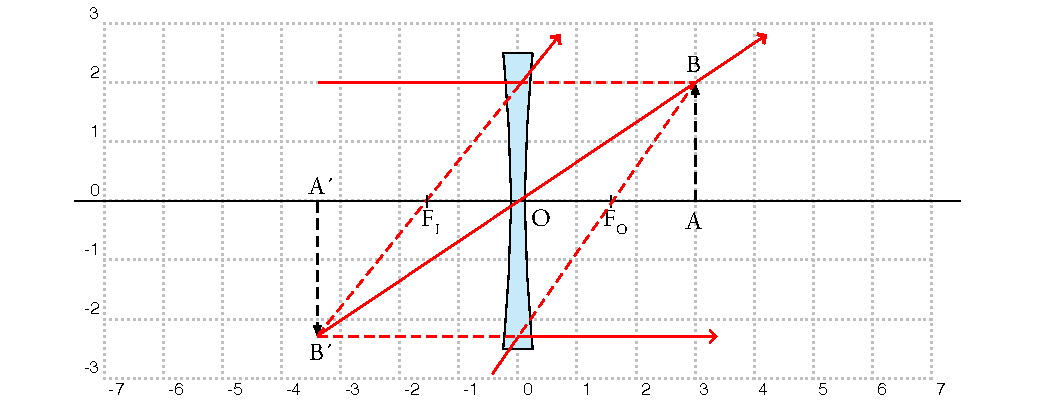
\includegraphics[width=0.7\textwidth]{./otica_images/7-DivVirtVirt}
	\caption{Lente divergente com objeto virtual e imagem virtual. \label{fig:DivVirtVirt}} 
\end{figure}

\subsubsection{\sf Lente divergente $f<0$ -- Imagem virtual}
A Fig. \ref{fig:DivVirtVirt} representa um objeto virtual ($d_O<0$, à direita da lente) para uma lente divergente ($f<0$)
e a correspondente imagem. Na situação da figura, o objeto está à direita do foco $F_O$: $|d_O|>|f|$. Verifica-se assim:

\begin{IEEEeqnarray}{rCl}
 d_O < 0 & &  f < 0   \nonumber\\
\frac{d_I}{|d_O|}  & =&  \frac{|f|}{|d_O| -|f|}     \nonumber
\end{IEEEeqnarray}

A imagem resultante é também virtual $d_I<0$, à esquerda da lente) e invertida ($A>0$), verificando-se as seguintes relações
em função da distância:
\begin{equation}
|d_O|  =  \left\{
\begin{array}{rl}
|d_O|   = |f|:  &   |d_I| \to \infty, \quad A \to \infty ,\\
|f| < |d_O|   < 2|f|:  &   |d_I|  > |d_O| , \quad A  >1  ,\\
|d_O|   = 2|f|:  &   |d_I| = |d_O|, \quad A =1  ,\\
|d_O|  > 2|f|:   & |d_I|  <|d_O| , \quad 0 < A  <1  .
\end{array}  \right.
%f<0 \quad \to   d_O> 0 ; \quad  d_I <0  
\end{equation}

%%%%%%%%%%%%%%%%%%%%%%%%%%%%%%%%%%%%%%%%%%%%%%%%%%
\subsubsection{\sf Lente divergente $f>0$ - Imagem real}

A Fig. \ref{fig:DivVirtReal} representa um objeto virtual ($d_O<0$, à direita da lente) para uma lente divergente ($f<0$)
e a correspondente imagem. Na situação da figura, o objeto está à esquerda do foco $F_O$: $|d_O|<|f|$. Verifica-se assim:

\begin{figure}[H]
	\centering 
	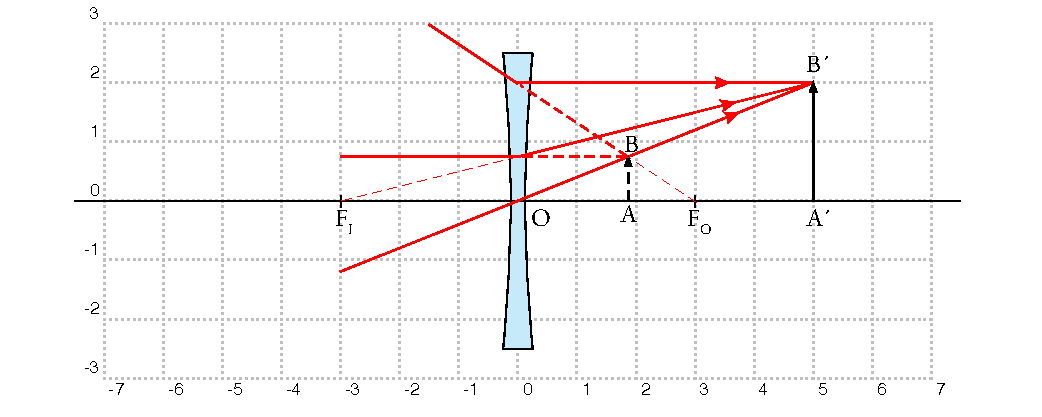
\includegraphics[width=0.7\textwidth]{./otica_images/8-DivVirtReal}
	\caption{Lente divergente com objeto virtual e imagem real. \label{fig:DivVirtReal}} 
\end{figure}

\begin{IEEEeqnarray}{rCl}
 d_O < 0 & &  f < 0   \nonumber\\
\frac{d_I}{|d_O|}  & =&  \frac{|f|}{|f|-|d_O|} \quad \to \quad A=\frac{d_I}{d_O} =\frac{f}{d_O-f}<0     \nonumber
\end{IEEEeqnarray}



A imagem resultante é agora real ($d_I>0$, à direita da lente) e direita ($A<0$), verificando-se as seguintes relações em
função da distância:
\begin{equation}
|d_O|  =  \left\{
\begin{array}{rl}
|d_O|   \to |f|:  &   |d_I| \to \infty, \quad A \to -\infty ,\\
|d_O|   = |f|/2:  &   |d_I| = f, \quad A =-2  ,\\
|d_O|  =0:  & |d_I|  =0 , \quad A=-1.
\end{array}  \right.
%f<0 \quad \to   d_O> 0 ; \quad  d_I <0  
\end{equation}



%%%%%%%%%%%%%%%%%%%%%%%%%%%%%%%%%%%%%%%%%%%%%%%%%%
%%%%%%%%%%%%%%%%%%%%%%%%%%%%%%%%%%%%%%%%%%%%%%%%%%

\section{\sf Associação de lentes delgadas}

Para duas lentes delgadas de distâncias focais $f_1$ e $f_2$ afastadas de $D$ (para $D \ll f_1,f_2$) pode calcular-se a
distância focal equivalente do conjunto através de: 

 \begin{equation}
	\label{eq:assoclentes}
    \fbox{
        $ \displaystyle
	\frac{1}{f_{equiv}} = \frac{1}{f_1} + \frac{1}{f_2} - \frac{D}{f_1 \,f_2} 
        $
    }
\end{equation}

A dificuldade
%quando se usa o método direto quer dos focos conjugados, para 
na determinação da distância focal equivalente ${f_{equiv}}$ é a medição das distâncias $d_O$ e $d_I$ 
(que são diferentes das distância do objeto e da imagem às superfícies das lentes ou aos seus planos médios).

Uma abordagem preferível consiste em usar a equação (\ref{eq:focosconjug}) separadamente para cada uma das lentes, e
considerar que a \emph{primeira imagem} (real ou virtual) irá constituir-se como o \emph{objeto} para a segunda lente.
Neste caso, as regras descritas acima para o traçado de raios de lentes individuais aplicam-se consecutivamente:
\begin{enumerate}
\item  A partir da posição do objeto $AB$ e do tipo da primeira lente $L_1$, determina-se a posição da imagem intermédia $A'B'$
\item  A partir da posição da imagem intermédia (agora tomada como objeto da segunda lente) e do tipo da segunda lente $L_2$,
determina-se a posição da imagem final $A''B''$
\end{enumerate}
Vamos aplicar este método para várias combinações de lentes convergentes e divergentes.

%%%%%%%%%%%%%%%%%%%%%%%%%%%%%%%%%%%%%%%%%%%%%%%%%%
\subsection{\sf Lente convergente - lente convergente}
A Fig. \ref{fig:DuplaConvConv1} representa duas lentes convergentes, $L_1$ e $L_2$, de distâncias focais $f_1$ e $f_2$
respectivamente, separadas de uma distância $D$. O objeto (real) $AB$ situa-se à esquerda de $L_1$, e tem uma imagem $A'B'$
por intermédio de $L_1$. Esta imagem constitui-se como objeto virtual para $L_2$, resultando no final a imagem $A''B''$.
Esta é a montagem mais simples de um \textbf{telescópio}, a partir do qual se podem obter grandes ampliações.

\begin{figure}[H] 
	\centering 
	\includegraphics[width=0.9\textwidth]{./otica_images/9-DuplaConvConv1}
	\caption{Sistema de duas lentes convergentes, com objeto intermédio real. \label{fig:DuplaConvConv1}} 
\end{figure}

Apliquemos as equações de lentes individuais para cada caso:

\begin{equation}
|d_O|  =  \left\{
\begin{array}{llll}
 \frac{1}{d_{O_1}} +  \frac{1}{d_{I_1}}   = \frac{1}{f_1}  & d_{O_1} = AO_1 & d_{I_1} = O_1A' & f_1 = O_1 F_{O_1} = O_1\,F_{I_1} \\
 \frac{1}{d_{O_2}} +  \frac{1}{d_{I_2}}   = \frac{1}{f_2}  & d_{O_2} = A'O_2 & d_{I_2} = O_2\,A'' & f_2 =  F_{O_2}\,O_2\, = O_2\,F_{I_2} \\
O_1\,O_2 = D = d_{I_1} + d_{O_2}
\end{array}  \right.
\label{eq:assoclentes_2}
\end{equation}

\begin{figure}[H]
	\centering 
	\includegraphics[width=0.9\textwidth]{./otica_images/10-DuplaConvConv2}
	\caption{Duas lentes convergentes, com objeto intermédio virtual. \label{fig:DuplaConvConv2}} 
\end{figure}

Estas três expressões permitem calcular o valor de uma das incógnitas, conhecidos os valores das outras. Por exemplo, uma
aplicação comum desta montagem consiste em determinar o valor de uma distância focal desconhecida $f_2$, conhecidos os valores
de $f_1$, $d_{O_1}$, $d_{I_2}$ e $D$.

As mesmas expressões aplicam-se para o caso de uma imagem obtida por uma lente $L_1$ que passa a ser um “objeto” virtual
para $L_2$, isto é, em que $d_{O2}<0$, situação ilustrada na Fig. \ref{fig:DuplaConvConv2}.



%%%%%%%%%%%%%%%%%%%%%%%%%%%%%%%%%%%%%%%%%%%%%%%%%%
\subsection{\sf Lente convergente - lente divergente}
O outro sistema de lente dupla de interesse é o caso em que temos uma lente convergente e uma divergente separadas de $D$,
ilustrado na Fig. \ref{fig:DuplaConvDiv1}, em que $L_1$ é convergente e $L_2$ é divergente. A lente $L_1$ produz uma imagem
intermédia $A'B'$ real e invertida, que é o objeto (real) de $L_2$. Uma vez que a segunda lente é divergente, a sua imagem
$A''B''$ (a imagem final) é sempre virtual e invertida.

\begin{figure}[H] 
    \centering 
	\includegraphics[width=0.9\textwidth]{./otica_images/11-DuplaConvDiv1}
	\caption{Sistema de lente convergente e divergente  com objeto intermédio real: a imagem final é virtual e invertida.
    \label{fig:DuplaConvDiv1}} 
\end{figure}

A Fig. \ref{fig:DuplaConvDiv2} ilustra a situação em que $A'B'$ está numa posição à direita de $L_2$: é uma imagem real
(de $L_1$) mas um objeto virtual (de $L_2$), já que $d_{O2}<0$. A imagem $A''B''$ resultante é real e invertida.

\begin{figure}[H] 
\begin{center}
	\includegraphics[width=0.9\textwidth]{./otica_images/12-DuplaConvDiv2}
	\caption{Sistema de lente convergente e divergente com objeto intermédio virtual: a imagem final é real e invertida. 
    \label{fig:DuplaConvDiv2}} 
\end{center}
\end{figure}

\begin{figure}[H]  
\begin{center}
	\includegraphics[width=0.9\textwidth]{./otica_images/13-DuplaConvDiv3}
\end{center}
	\caption{Sistema de lente convergente e divergente.  \label{fig:DuplaConvDiv3}} 
\end{figure}


Por fim, se nesta montagem permutarmos $L_1$ e $L_2$ (Fig. \ref{fig:DuplaConvDiv3}), obtém-se também uma imagem real  $A''\,B''$, desde que a distância $d_{O1}=A\,O_1$ seja idêntica.
Em qualquer destas situações, pode sempre calcular-se $f_2 < 0$ usando o conjunto das três equações (\ref{eq:assoclentes_2}).
\clearpage

%%%%%%%%%%%%%%%%%%%%%%%%%%%%%%%%%%%%%%%%%
%%%%%%%%%%%%%%%%%%%%%%%%%%%%%%%%%%%%%%%%%
%%%%%%%%%%%%%%%%%%%%%%%%%%%%%%%%%%%%%%%%%


\section{\sf Instrumentos óticos}
Um instrumento ótico é um dispositivo baseado nos princípios da ótica cujo objectivo é auxiliar a visão humana. Nestes sistemas, designamos por \emph{objectiva} a lente que está do lado do objeto AB e por \emph{ocular} aquela que está do lado do observador, com distâncias focais $f_{obj}$ e $f_{ocu}$ respetivamente. Em ambos os casos, a ocular está  próxima da \emph{imagem intermédia} A'B' formada pela objectiva. Sendo a distância inferior à distância focal $f_{ocu}$, a imagem final será \emph{virtual}, ou seja, visível apenas através da lente.
Assim, o papel da ocular consiste em ampliar a imagem intermédia, tal como um lupa amplia um objeto.

\subsection{\sf O olho humano}
Vamos primeiro abordar a fisiologia do olho humano (Fig. \ref{fig:olho-1}) para compreender as suas limitações.
Este pode ser considerado como um sistema ótico que projecta imagens (reais) dos objetos exteriores na retina,
através de duas lentes convergentes: a córnea e o cristalino. Para o nosso estudo, vamos considerar que estas
lentes são substituídas por um sistema equivalente constituído por uma única lente, com o máximo de distância focal $f$
igual a 2,5 cm, que é a média da distância entre a córnea e a retina. A potência em dioptrias (dt) desta lente
equivalente é dada por:

\begin{equation}
D=\frac{1}{f} \,[\mathrm{m}^{-1}] = \frac{1}{0,025} \,[\mathrm{m}^{-1}] = 40 \,[\mathrm{m}^{-1}]=40\, \mathrm{dt}.
\end{equation}

\begin{figure}[H]
	\centering 
	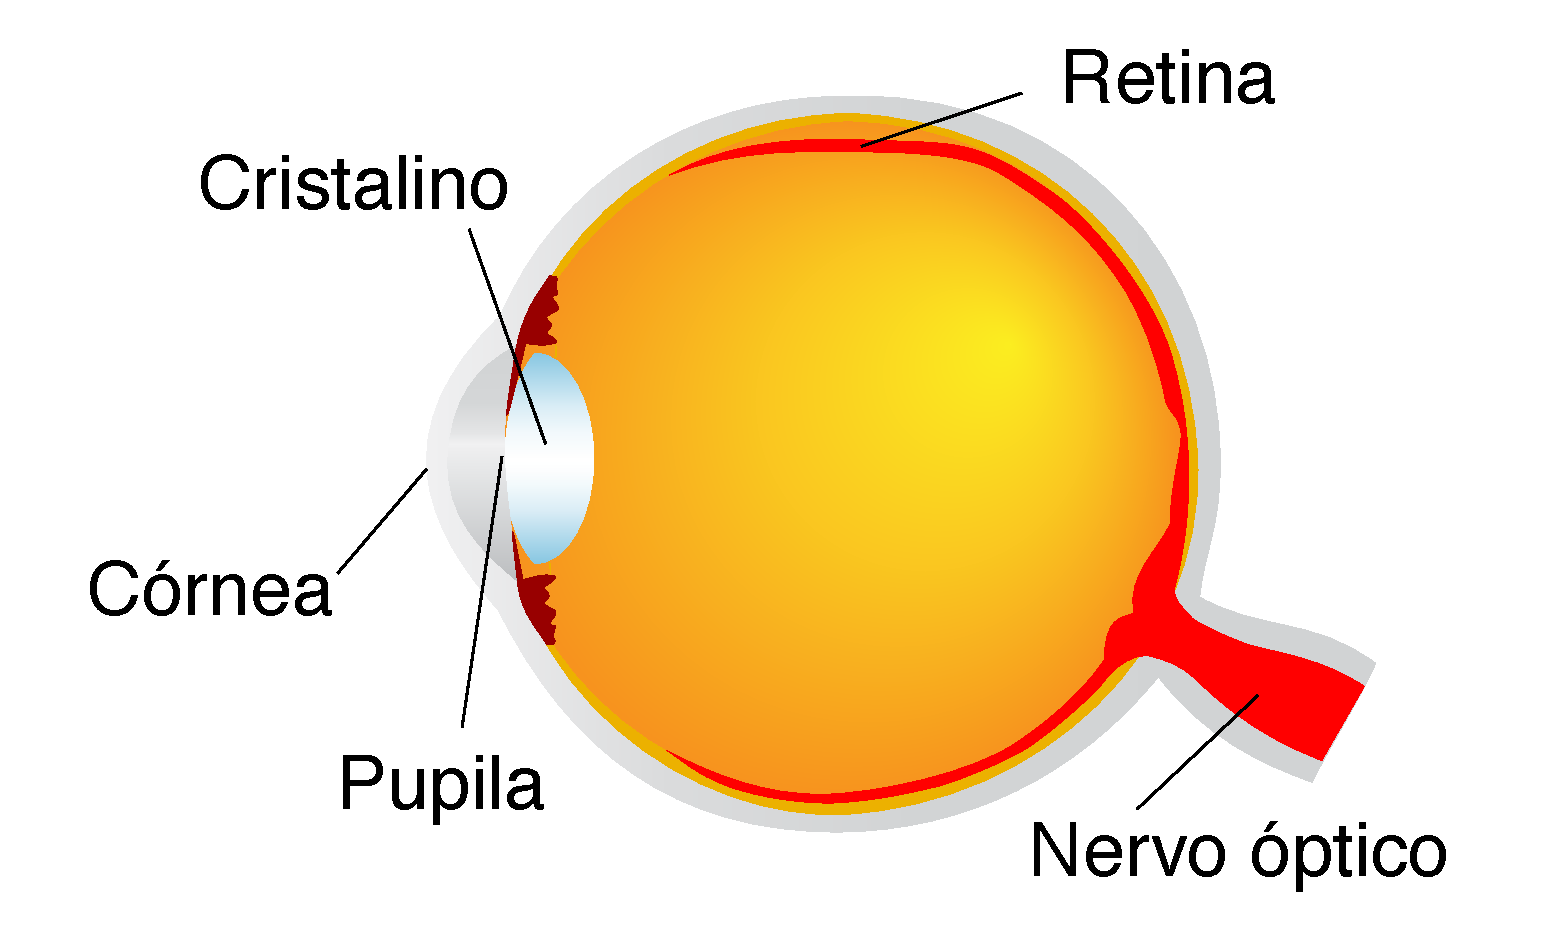
\includegraphics[width=0.5\textwidth]{./otica_images/olho-1}
	\caption{Diagrama dos principais elementos do olho humano. \label{fig:olho-1}} 
\end{figure}


Para uma pessoa com visão normal ou munida de correção adequada (óculos graduados ou lentes de contacto), os raios óticos
provenientes de um objeto no infinito\footnote{Para efeitos práticos, considera-se o infinito óptico qualquer distância
superior a 5 m.} chegam paralelos ao olho e são focados na retina sem necessidade de esforço, ou seja, com o olho relaxado
(Fig. \ref{fig:olho-2} à esq.). à medida que o objeto se aproxima do olho, é necessário os músculos ciliares aumentarem a
curvatura da lente para criar uma imagem focada na retina -- a isto chama-se \emph{acomodação do olho}. O ponto mais próximo
do olho para o qual a lente ainda consegue focar a imagem na retina é designado por \emph{ponto próximo} (Fig. \ref{fig:olho-2} à dir.)
e considera-se igual a 0,25 m para uma visão normal padrão, valor que tem tendência a aumentar com a idade.

\begin{figure}[H]
	\centering 
	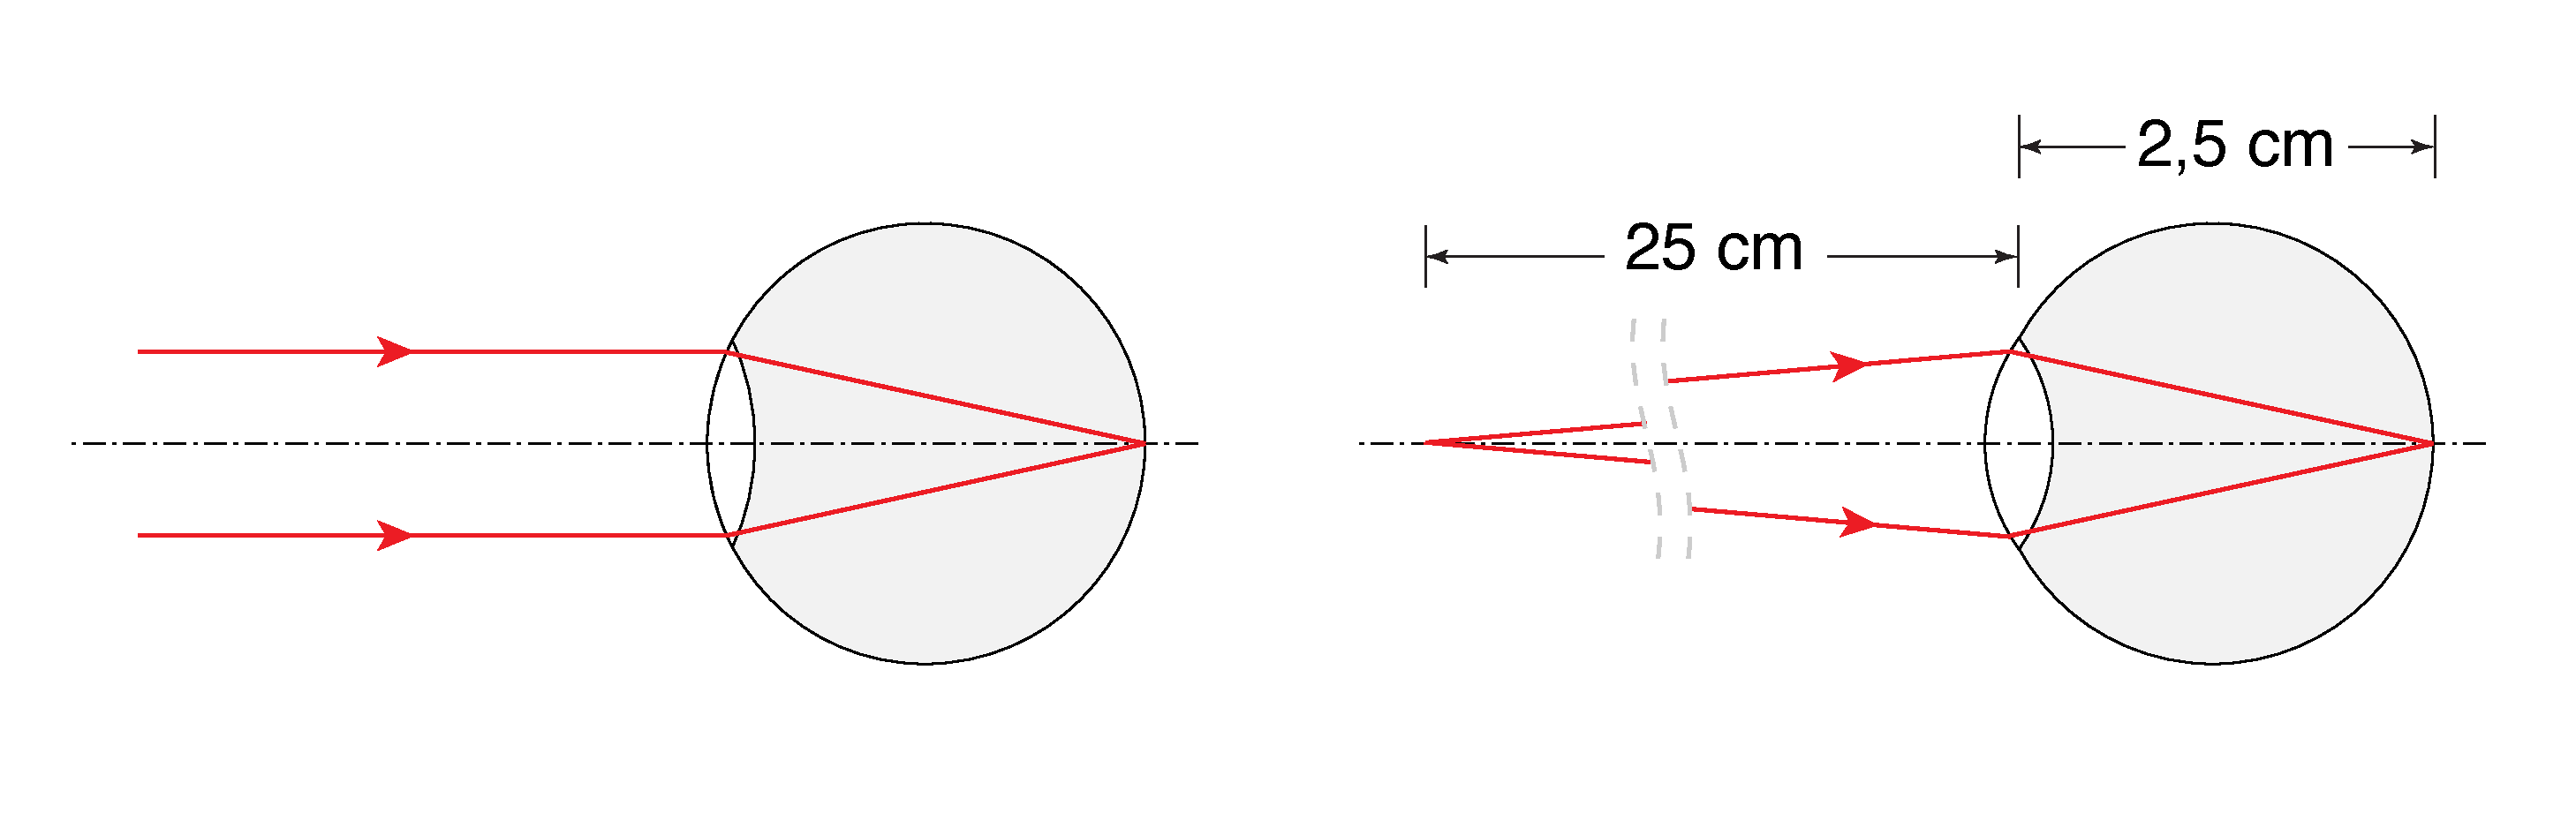
\includegraphics[width=0.9\textwidth]{./otica_images/olho-2}
	\caption{Esquema do olho no caso de objetos no infinito (esq.) e no ponto próximo (dir.). \label{fig:olho-2}} 
\end{figure}

O tamanho aparente dum objeto é determinado pelo tamanho que a imagem apresenta na retina. Mesmo sem variar o tamanho
real do objeto, este pode ser visto maior se o aproximarmos do olho, porque o tamanho da sua imagem na retina é maior.
A avaliação do tamanho da imagem na retina pode ser feita através da medição do ângulo $\theta$, que corresponde à inclinação
dos raios principais do extremo da imagem (Fig. \ref{fig:olho-3}).

\begin{figure}[H]
	\centering 
	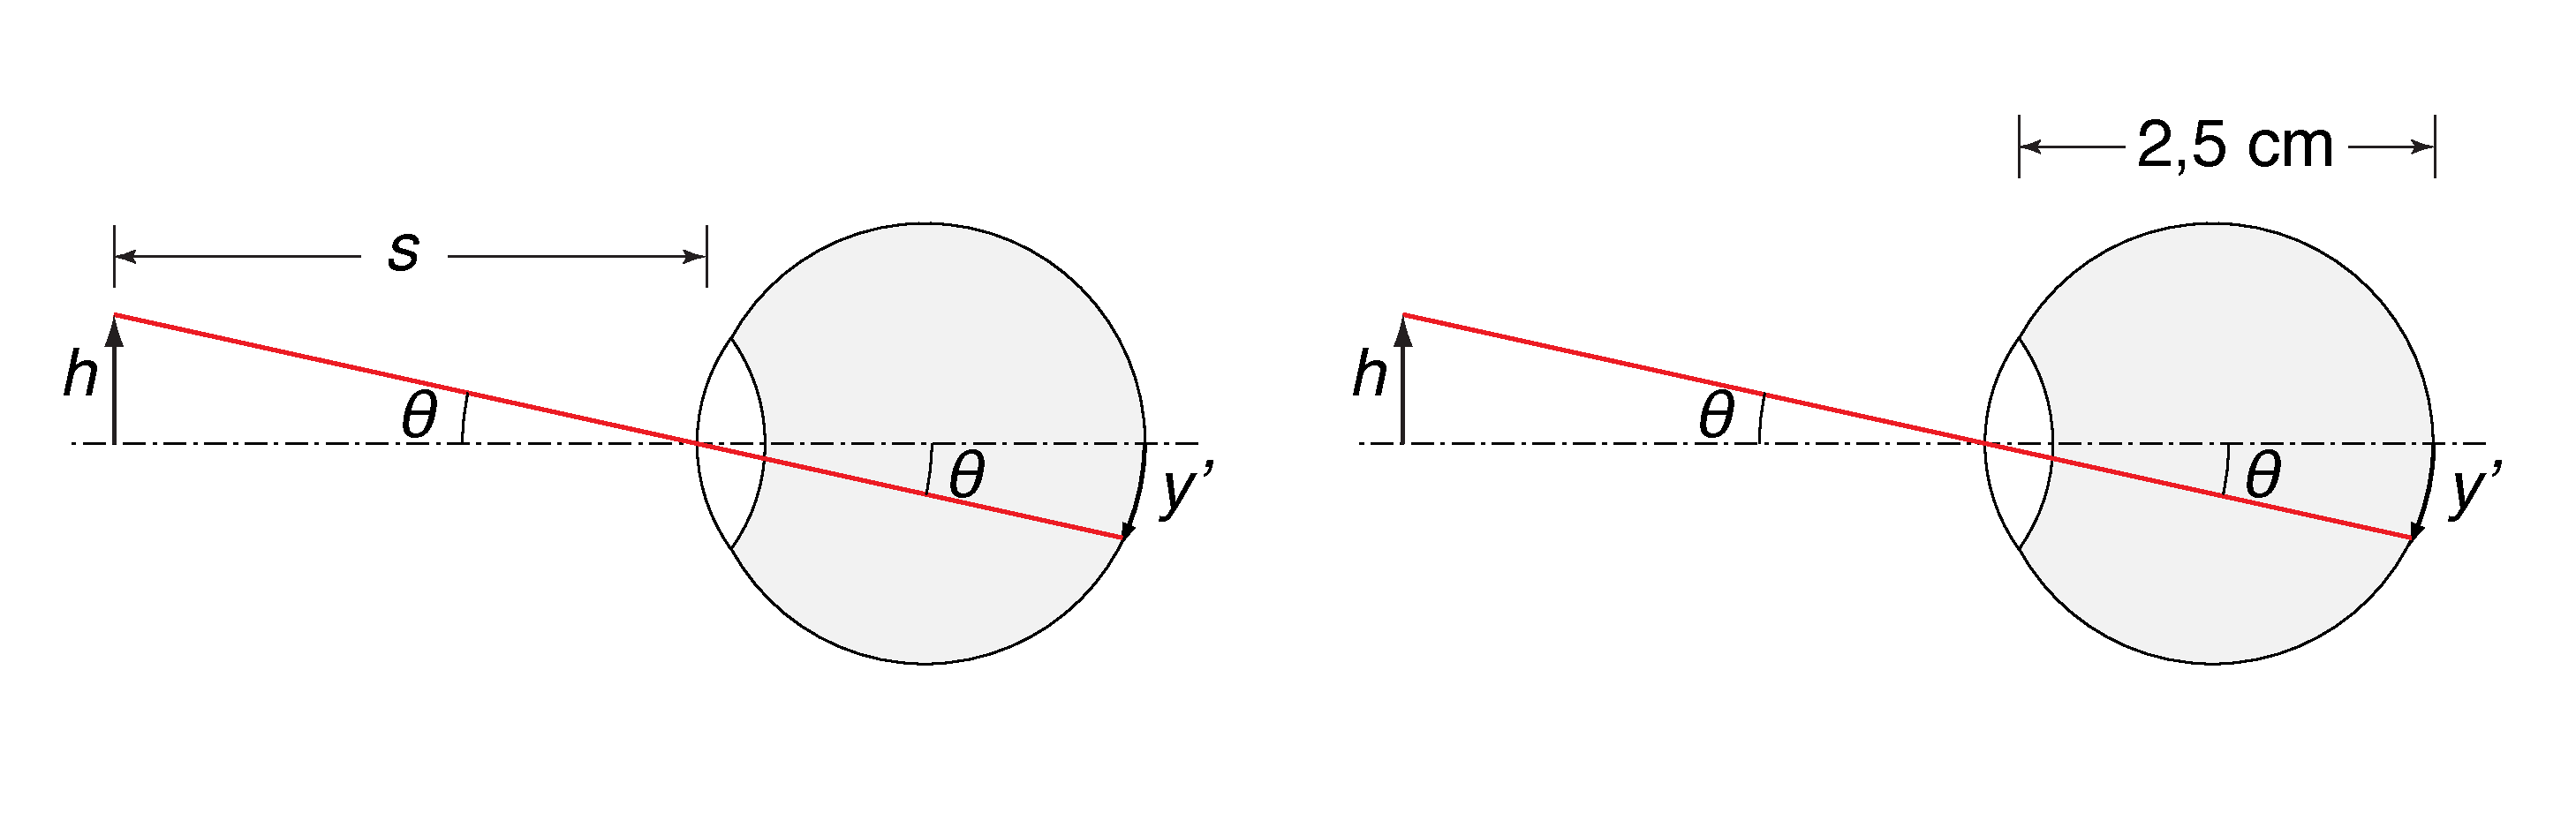
\includegraphics[width=0.9\textwidth]{./otica_images/olho-3}
	\caption{Formação de imagem na retina de um objeto de altura $h$ a uma distância $s$. \label{fig:olho-3}} 
\end{figure}

Considere-se um objeto com altura $h$ a uma distância $s$ do olho. Para o objeto podemos escrever $\tan\theta=h/s$.
Para a imagem na retina, de altura $y'$, vem $\tan\theta = y' /$(2,5 cm). Na aproximação paraxial, ou seja de ângulos pequenos,
podemos usar $\tan\theta \approx\theta$, e assim $\theta\approx h/s=y'/$(2,5 cm). Desta relação conclui-se que $y'$ é proporcional
a $h$, tamanho do objeto, e inversamente proporcional à distância $s$ entre o objeto e o olho. 


O princípio dos instrumentos óticos consiste no aumento do tamanho da imagem na retina, $y'$, permitindo assim visualizar objetos
muito pequenos ou afastados. Do exposto acima, podemos concluir que a sua operação baseia-se na criação de uma imagem (real ou virtual)
com um tamanho aparente maior que $h$ e/ou 
 a uma distância aparente inferior a $s$. Em qualquer dos casos, a imagem final produzida deverá estar situada além do
 ponto próximo, caso contrário não conseguirá ser focada.


%%%%%%%%%%%%%%%%%%%%%%%%%%%%%%%%%%%%%%%%%
\subsection{\sf Lupa}

A lupa simples é o instrumento ótico mais elementar. Consiste numa só lente convergente e permite aumentar o tamanho
aparente do objeto, ou seja, o tamanho da imagem na retina. Sabendo que a maior imagem que se pode obter dum objeto
com o olho desarmado é quando o objeto está no ponto próximo (Fig. \ref{fig:olho-4}), e dado que $y'_0$, tamanho da
imagem na retina, é proporcional ao ângulo definido entre a altura do objeto $h_0$ e a sua distância ao olho,
pode-se escrever a relação

\begin{equation}
\theta_0=h_0/0,25
\end{equation}

Na visão auxiliada pela lupa, esta é colocada perto do olho, e o objeto colocado a uma distância inferior ao foco. A imagem
produzida pela lupa é virtual, ampliada e direita.

\begin{figure}[H]
	\centering 
	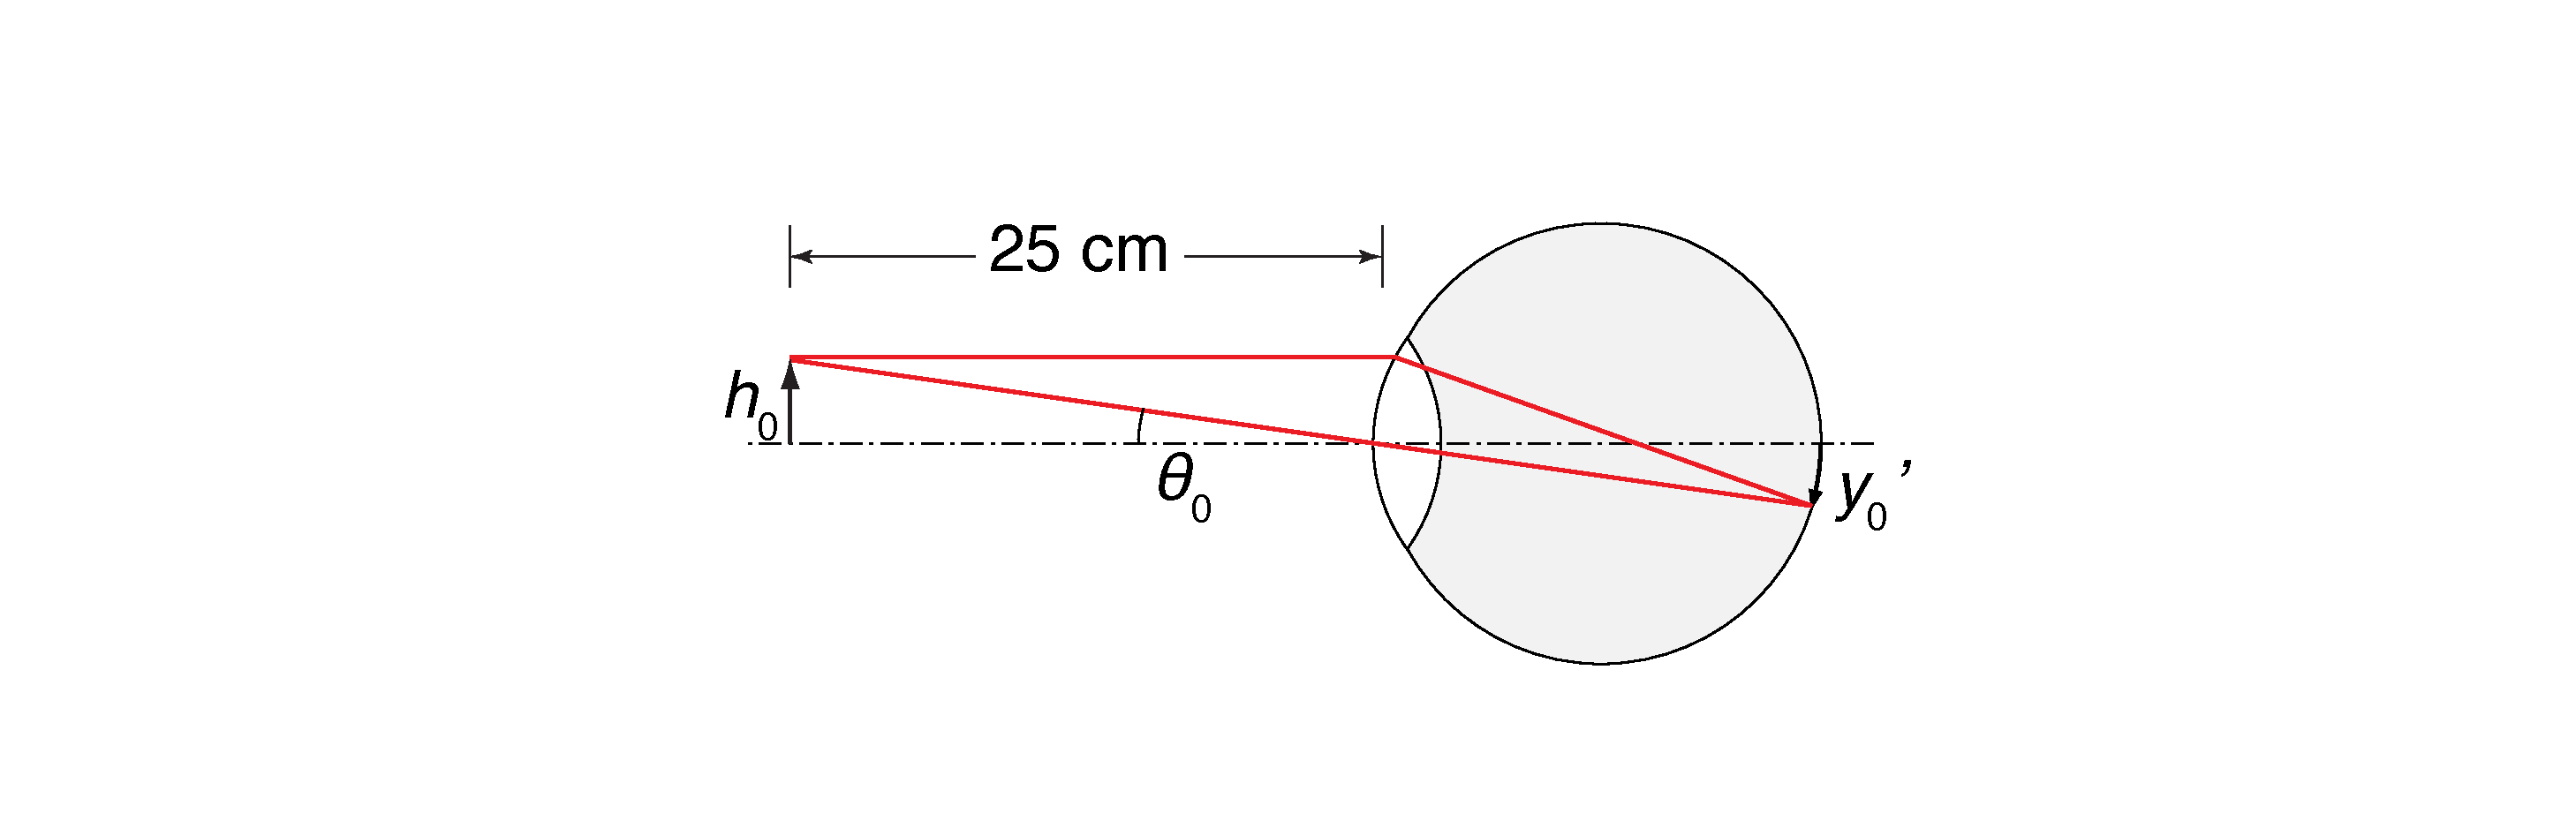
\includegraphics[width=0.8\textwidth]{./otica_images/olho-4}
		\caption{objeto no ponto próximo visto pelo olho desarmado. \label{fig:olho-4}} 
\end{figure}



\begin{figure}[H]
	\centering 
	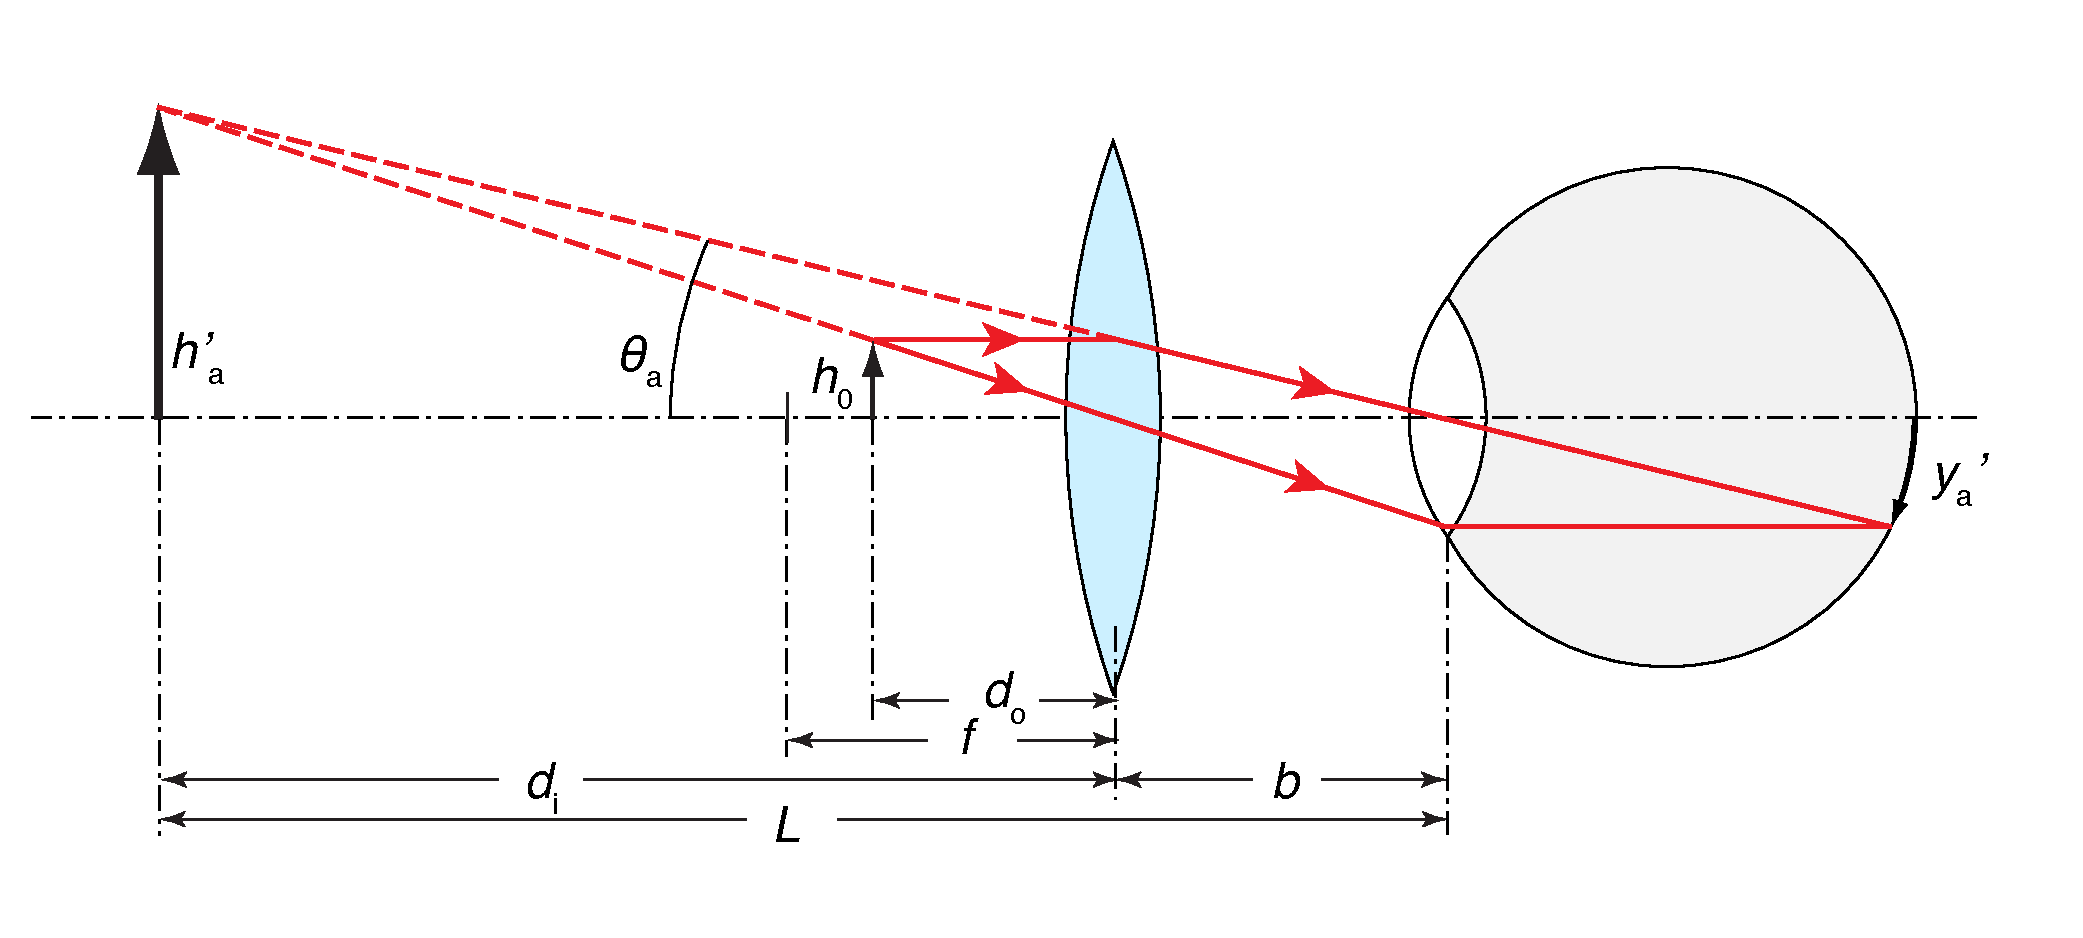
\includegraphics[width=0.8\textwidth]{./otica_images/olho-5}
	\caption{Formação de imagem com o auxílio de uma lupa a uma distância $b$ do olho. O objeto $h_0$ está a uma distância
    $d_O<f$ da lente, e a imagem (virtual) $h'_a$ aparenta estar a uma distância $d_i$ da lente e $L$ do olho. \label{fig:olho-5}} 
\end{figure}

\subsubsection{ \sf Ampliação angular}

A \emph{ampliação angular} $M_A$ dum instrumento óptico é determinada pela razão entre $y'_a$, dimensão da imagem na retina
quando o objeto é visto através do instrumento (Fig. \ref{fig:olho-5}), e $y'_0$, dimensão da imagem na retina quando vista
pelo olho desarmado e o objeto no ponto próximo. A razão entre os respectivos ângulos permite esse cálculo, isto é 

\begin{equation}
M_A=\frac{y'_a}{y'_0}=\frac{\theta_a}{\theta_0}
\end{equation}

Tirando partido da aproximação paraxial, temos $\tan\theta_a = h'_a / L \approx \theta_a$ e $\tan\theta_0 = h_0 / 0,25 \approx\theta_0$, portanto pode-se escrever a ampliação angular como:

\begin{equation}
M_A = \frac{h'_a/L}{h_0/0,25}=-\frac{d_i\,0,25}{d_0 L}= \frac{0,25}{L}\left(1-\frac{d_i}{f}\right) 
\end{equation}

onde na última igualdade se recorreu à equação dos focos conjugados. Como a distância à imagem é negativa, $d_i = - (L – b)$,
obtém-se por fim

\begin{equation}
M_A = \frac{0,25}{L}\left(1+\frac{L–b}{f}\right)
\end{equation}

Da análise desta expressão pode-se dizer que a ampliação diminui se $L$ ou $b$ aumentam. Existem três casos particulares de ampliação:

\begin{enumerate}

\item  Se $b=f \to M_A = \frac{0,25}{f}=0,25D$, em que $D$ é a potência da lupa em dioptrias.

\item  Se $b=0\to M_A = 0,25\left(\frac{1}{L}+\frac{1}{f}\right)$.
Se $b= 0$ e também $L = 0,25 $ m (valor mínimo para $L$, uma vez que a imagem também deve poder ser focada correctamente pelo olho),
então obtém-se para $M_A$ o valor máximo, igual a $M_A = 1+\frac{0,25}{f}= 1+0,25D$. Este caso corresponde a ter a lupa "encostada"
ao olho, e a imagem aumentada surge à distância do ponto próximo.

\item  Se o objeto é colocado no foco ($d_O=f$), então a lupa forma a sua imagem no infinito $(L = \infty)$ e a ampliação é 
\begin{equation*}
M_A = \lim_{L\to\infty}\frac{0,25}{L}\left(1+\frac{L–b}{f}\right)= \frac{0,25}{f}=0,25D
\end{equation*}
Neste caso, o olho recebe raios paralelos e não necessita de fazer acomodação, o que é mais cómodo, e a ampliação apenas
se reduz de uma unidade relativamente ao caso 2.
\end{enumerate}

Exemplo: uma lente com $D=10$ dioptrias tem uma distância focal $f=10$ cm, e para $L=\infty$ tem uma ampliação de $M_A=$2,5 vezes.


%%%%%%%%%%%%%%%%%%%%%%%%%%%%%%%%%%%%%%%%%
% \subsection{\sf Microscópio composto}

% O microscópio é o instrumento óptico empregado para observar objetos pequenos, colocados muito próximos do instrumento.
% Na sua forma mais simples, consiste em duas lentes convergentes. A lente mais próxima do objeto (\emph{objectiva}) tem uma
% distância focal $f_{obj}$, menor que a distância focal $f_{ocu}$ da lente mais perto do olho (\emph{ocular}) (Fig. \ref{fig:microscopio}).

% \begin{figure}[H]  \centering 
% 	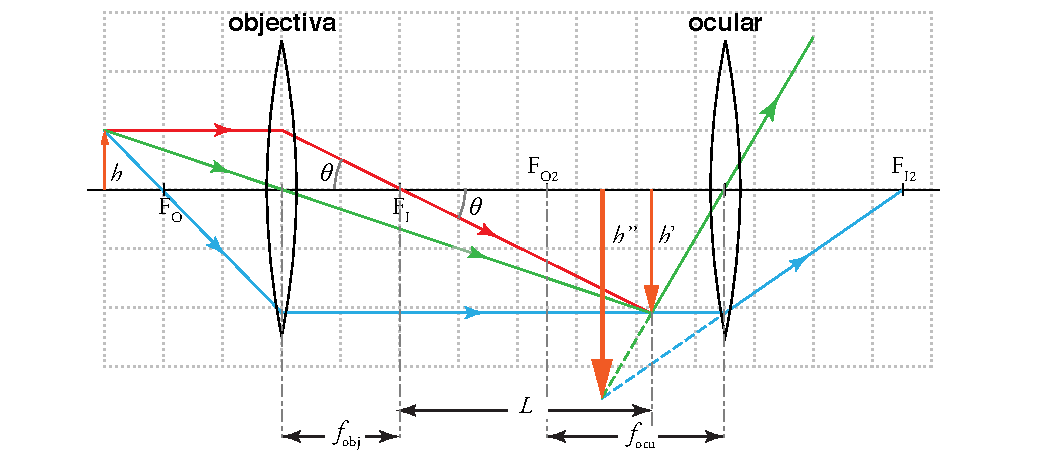
\includegraphics[width=0.9\textwidth]{./otica_images/microscopio}
% 		\caption{Formação de imagem num microscópio. \label{fig:microscopio}} 
% \end{figure}

% Um objeto de altura $h$ é colocado, em relação à objectiva, mais afastado do que o foco desta, produzindo uma imagem de
% tamanho $h'$ que é real, invertida e maior que o objeto. A objectiva produz assim uma imagem com
% \emph{ampliação transversal linear} $M_T$,\footnote{Conforme vimos atrás, para o caso de uma única lente esta ampliação
% é designada $A$.} dada por:

% \begin{equation}
% M_T=\frac{h'}{h} = -\frac{L\tan\theta}{f_{obj}\tan\theta}= -\frac{L}{f_{obj}}
% \end{equation}

% O sinal negativo indica que a imagem é invertida e, uma vez que é real, a imagem pode ser projectada sobre um alvo para
% se medir o seu tamanho.

% A lente ocular é usada para aumentar a imagem formada pela lente objectiva. Assim, a ocular é colocada de modo a que a
% imagem $h'$ produzida pela objectiva (agora \emph{objeto virtual} da segunda lente) venha localizar-se a uma distância
% ligeiramente inferior ao seu foco $f_{ocu}$. Nesta condição, a ocular actua como uma simples lupa, que permite trazer o
% objeto $h’$ para uma distância mais curta do que o ponto próximo (0,25 m), e produz a imagem $h''$. A \emph{ampliação final} $M$
% é dada pelo produto da ampliação transversal para a lente objectiva e a ampliação angular $M_A$ obtida para a lente ocular.
% No caso da lente ocular estar encostada ao olho, como é habitual num microscópio, estamos no caso $b=0$ e, das expressões
% anteriores para a ampliação linear e angular, obtemos

% \begin{equation}
% M = \frac{h''}{h}=M_T\times M_A.
% \end{equation}




%%%%%%%%%%%%%%%%%%%%%%%%%%%%%%%%%%%%%%%%%%%%%%%%%%
\newpage
\section{\sf Procedimento experimental}


\subsection*{\sf Material}
Caixa de ótica equipada com
\begin{itemize}
\item calha graduada
\item fonte luminosa com lâmpada de incandescência linear
\item lentes convergentes e divergente
\item semi-cilindro de vidro acrílico
\item diafragmas
\item polaroides
\item suportes
\end{itemize}


\subsection*{\sf Trabalho preparatório} 
\begin{enumerate}
\item Preencha os objectivos do trabalho que irá realizar na sessão de laboratório. 
\item Preencha o quadro com as equações necessárias para o cálculo das grandezas, bem como as suas incertezas. 
\end{enumerate}
%%%%%%%%%%%%%%%%%%%%%%%%%%%%%%%%%%%%%%%%%%%%%%%%%%

\subsection{\sf  Determinação do índice de refracção dum vidro acrílico }
\subsubsection*{\sf Alinhamento}
\begin{enumerate}
\item Monte a fonte luminosa numa das extremidades da calha graduada e ligue a lâmpada.
\item Utilizando uma lente, obtenha  um  feixe  de  luz  branca  de  raios  paralelos. De que tipo de lente necessita?
\item Com os diafragmas, obtenha um feixe de luz estreito ($\approx$ 1 mm), alinhado com o eixo da calha graduada.
Verifique que a espessura do feixe de luz se mantém tão constante quanto possível ao longo de toda a calha.
\end{enumerate}

\subsubsection*{\sf Face plana}
\begin{enumerate}
 \setcounter{enumi}{3}
\item Monte o suporte com o círculo graduado e o semi-cilindro  de  vidro  acrílico centrado, de modo a que o feixe de luz
branca incida na sua superfície  plana.  Observe  e obtenha os ângulos de reflexão e de transmissão para vários valores dos
ângulos do feixe incidente, à esquerda e à direita.  Registe medições  para, pelo  menos,  nove  valores  diferentes  do
ângulo de incidência.
\item Represente as medições num gráfico e, a partir deste, determine por ajuste o índice de refracção do vidro acrílico. 
Anexe o gráfico ao relatório.
\end{enumerate}

\subsubsection*{\sf Face cilíndrica}
\begin{enumerate}
 \setcounter{enumi}{5}
\item Rode o círculo graduado de modo a que o feixe de luz incida na  superfície cilíndrica do vidro acrílico. Repita 
as  medidas  e  a  análise  dos  resultados. 
\end{enumerate}

\subsubsection*{\sf Ângulo-limite}
\begin{enumerate}
 \setcounter{enumi}{6}
 \item Estime o valor do índice de refracção a partir do ângulo limite de reflexão total. 
\item  Para o desvio à exatidão, considere como exato o valor médio das medições anteriores. 
\item Nas suas conclusões, compare os valores obtidos  para $n_{vidro}$ e a sua precisão 

\end{enumerate}

%%%%%%%%%%%%%%%%%%%%%%%%%%%%%%%%%%%%%%%%%%%%%%%%%%
\subsection{\sf Polarização da luz. Ângulo de Brewster}
\begin{enumerate}
\item Observe o efeito de interposição de dois filtros polarizadores, paralelos ou cruzados, no percurso de um feixe luminoso. 
\item Usando a mesma montagem do ponto anterior, polarize o feixe paralelamente ao plano
de incidência, orientando o eixo $0^\circ-180^\circ$ do filtro polarizador na vertical. 
\item A partir  do valor médio obtido para o índice de refracção (o que usou na secção anterior), calcule o valor "teórico"
do ângulo de Brewster e verifique experimentalmente que, para esse valor, os raios reflectido e transmitido fazem 90$^\circ$ entre si. 
\item Para ângulos de incidência próximos do ângulo de Brewster, obtenha o  intervalo angular em que praticamente  se extingue
o feixe reflectido. 
\end{enumerate}

%%%%%%%%%%%%%%%%%%%%%%%%%%%%%%%%%%%%%%%%%%%%%%%%%%
\subsection{\sf Distância focal de uma lente convergente ( $f  \approx$ 75 mm) }
 
\begin{enumerate}
\item Obtenha  um  feixe  de  luz  branca  de  raios  paralelos, usando a lente colimadora.
\item Seleccione a lente de distância focal mais curta e determine o seu valor pelo método directo. Repita a experiência
duas  vezes,  colocando  a  lente 
noutra posição relativamente à lente de raios paralelos. 
\item Retire a lente colimadora e coloque o \emph{objeto} com mira no suporte da calha, iluminando-o directamente com a fonte luminosa. Coloque a mesma lente convergente a uma distância 150 mm $> d_O >$ 75 mm do objeto.

\item Com o écran plano, procure a posição correcta para obter uma \emph{imagem} focada.
Utilizando a equação dos focos conjugados, calcule de novo a d.f. da lente. 
\item Na folha quadriculada em anexo, desenhe um diagrama com o eixo ótico, o objeto e a lente convergente. Utilizando as aproximações paraxial e das lentes delgadas, desenhe a construção geométrica e obtenha a posição da imagem e a respectiva ampliação.

\item Medindo agora a imagem, determine a ampliação linear. Compare-a com a que podia  calcular pelas distância $d_O$  e $d_I$. 
\item Repita a experiência, colocando a lente noutra posição relativamente ao objeto.  
\item Compare o valor da distância focal com o obtido em (1) e estime a precisão envolvida em 
cada um dos métodos que utilizou. 
\end{enumerate}

%%%%%%%%%%%%%%%%%%%%%%%%%%%%%%%%%%%%%%%%%%%%%%%%%%
\subsection{\sf   Distância focal de uma lente divergente ( $f  \approx$ --150 mm) }
\begin{enumerate}
\item Associe  no  mesmo  suporte  a  lente  divergente  com  uma  convergente ($f  \approx$ 75 mm), de  forma a  que  o 
par se comporte como um sistema convergente (com $D\approx 10$ mm). Escolha uma distância ao objeto $D_O$ adequada e utilize esta montagem para determinar a distância focal da lente divergente.
\item Repita a montagem para uma diferente distância ao objeto. 
\end{enumerate}

%%%%%%%%%%%%%%%%%%%%%%%%%%%%%%%%%%%%%%%%%%%%%%%%%%

% \subsection{\sf Microscópio composto}

% \subsubsection*{\sf Material}
% \begin{itemize}
% \item Lente objectiva $f$ = 75 mm e lente ocular $f$ = 150 mm
% \end{itemize}

% \subsubsection*{\sf Medição da ampliação angular da ocular}
% \begin{enumerate}
% \item Monte um ecrã graduado (E1) na parte lateral exterior de um suporte a $d_i\approx 25$ cm da extremidade da calha, de
% modo a ficar no ponto próximo do observador. Este ecrã será a \emph{escala de referência}, desempenhando o mesmo papel que a
% escala na parede, no caso do telescópio.
% \item Monte a lente ocular junto à mesma extremidade da calha, de modo a obter a condição $b\sim 0$ (verifique a Fig. \ref{fig:olho-5}). Calcule qual a distância $d_o$ dessa lente a que deverá colocar um objeto (altura $h_O$) de modo a que a sua imagem surja no ponto próximo. Use o valor obtido para determinar a ampliação angular (calculada).
% \item Coloque outro ecrã graduado (E2) entre a lente e E1, próximo da posição $d_o$ calculada acima, de modo a conseguir
% visualizar simultaneamente (a) a escala de E2 através da lente, com o olho esquerdo, e (b) a escala de E1 com o olho direito.
% \item Ajuste a posição de E2 até conseguir focar simultaneamente as imagens em ambos os olhos. Sobrepondo visualmente as duas
% escalas graduadas, meça o tamanho aparente $h'_a$ da imagem (virtual) de E2 e determine a ampliação angular $M_A$ da lente,
% usando a expressão adequada para esta configuração (ver Fig. \ref{fig:micro-composto})
% % \item Na folha quadriculada em anexo desenhe um diagrama de traçado de raios, com o objeto a uma distância do foco igual $\approx f/5$. Obtenha a posição da imagem intermédia e da imagem final.
% \end{enumerate}

% \begin{figure}[H]
% \begin{center}
% 	\includegraphics[width=0.45\textwidth]{micro-composto}
%     \caption{Esquema para a medição da ampliação angular da ocular.}
%     \label{fig:micro-composto}
% \end{center}
% \end{figure}

% \subsubsection*{\sf Medição da ampliação linear da objectiva}
% \begin{enumerate}
%     \item Mantendo a ocular montada e usando como referência a Fig. \ref{fig:microscopio}, junte uma objectiva e um objeto
%     (um écran graduado iluminado). Escolha uma altura $h_0$ adequada.
%     \item Se necessário, ajuste a objectiva para observar uma imagem focada através da ocular.
%     \item Com um ecrã auxiliar, observe a imagem intermédia $h'$ e meça a sua ampliação.
%     \item Calcule a ampliação final do microscópio composto.
% \end{enumerate}

\newpage

\end{document}